\documentclass[
  manuscript=article,  %% article (default), rescience, data, software, proceedings, poster
  layout=preprint,  %% preprint (for submission) or publish (for publisher only)
  year=20xx,
  volume=x,
]{extra/joas}

% --- blew is the area for authors ---

% remove the following two packages, and delete all \blindtext commands
\usepackage[english]{babel} 
\usepackage{blindtext}


% Make sure your article tile is within 12 words
\title{Using a concise title for your article}

\author{The Author name}
\affiliation{Institution-1, City, Country}

% maximum five keywords
\keywords{keyword; keyword-two; keyword number three} 

% Important: don't over use abbreviations. Only use abbreviation if the term is used more than ten times throughout the paper. Otherwise, write them in full.
% \abbreviations{
%     JOAS: Journal of Open Aviation Science, 
%     ATM: Air Traffic Management
% }


\begin{document}

\begin{abstract}
  An abstract summarizes in one paragraph with 300 words or less, the major aspects of the entire paper. They often include: 1) the overall purpose of the study and the research problem you investigated; 2) the basic design of you research approach; 3) major findings as a result of your analysis; and, 4) a brief summary of your interpretations and conclusions. 
\end{abstract}


\section{Introduction}

\blindtext 
open data in science \cite{murray2008open}. 


\blindtext [2]


\section{Method}

\subsection{Method part 1}

\blindtext The end result is in Figure.

\begin{figure}[ht!]
  \centering
  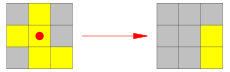
\includegraphics[width=0.45\textwidth]{./extra/1.png}
  \caption{An Example Figure}
  \label{fig:logo}
\end{figure}

\blindtext\footnote{This is how a footnote works.}

\subsection{Method part 2}

\subsubsection{Method part 2-1}

\blindtext Reference to Equation.

\begin{equation} \label{eq:cauchy_momentum}
\rho\frac{\mathrm{D} \mathbf{u}}{\mathrm{D} t} = - \nabla p + \nabla \cdot \boldsymbol \tau + \rho\,\mathbf{g}
\end{equation}


\subsubsection{Method part 2-2}

\blindtext Table shows an example.

\begin{table}[H]
  \centering
  \small
  \caption{Example table}
  \label{tb:example_table}
  \begin{tabular}{lll}
  \toprule
  \textbf{Parameter} & \textbf{Notation} & \textbf{Remarks} \\
  \midrule
  name & - & engine common identifier \\
  manufacture & - & name of the manufacture  \\
  bpr & $\lambda$ & bypass ratio \\
  pr & - & pressure ratio \\
  thrust & $T_0$ & maximum static thrust\\
  \bottomrule
  \end{tabular}
\end{table}

\blindtext


\section{Discussions}

\paragraph{Paragraph title} This is the paragraph with title if you want to use such function in the paper. \blindtext


\section{Reference}
\renewcommand{\section}[2]{} 
\begin{thebibliography}{20}

   \bibitem{1} Oluwaniyi O ,Zhang Y ,Gholizadeh H , et al.Correlating Groundwater Storage Change and Precipitation in Alabama, United States from 2000–2021 by Combining the Water Table Fluctuation Method and Statistical Analyses[J].Sustainability,2023,15(21).

  \end{thebibliography}


\end{document}